% Originally from a LyX file
\documentclass[english,conference,10pt]{IEEEtran}
\usepackage[T1]{fontenc}
\usepackage[utf8]{inputenc}
\usepackage{babel}
\usepackage{amsmath}
\usepackage{amsfonts}
\usepackage{amssymb}
\usepackage{units}
\usepackage{graphicx}
\usepackage{subcaption}
\usepackage{url}
\usepackage[capitalise]{cleveref}
\crefname{equation}{}{}
\begin{document}

\title{Daala: Building A Next-Generation Video Codec From Unconventional
Technology}


\author{\IEEEauthorblockN{Jean-Marc Valin, Timothy B. Terriberry, Nathan Egge, Thomas Daede,\\
Yushin Cho, Christopher Montgomery, Michael Bebenita}\\
\IEEEauthorblockA{Mozilla, Mountain View, USA}
\IEEEauthorblockA{Xiph.Org Foundation, USA}
jmvalin@jmvalin.ca
}
\maketitle
\begin{abstract}
Daala is a new royalty-free video codec that attempts to compete with
state-of-the-art royalty-bearing codecs. The main strategy for achieving this
goal is to use technology that is as different as possible from traditional
approaches used in video coding.
\end{abstract}


\section{Introduction}

Daala is a royalty-free video codec designed to avoid traditional
patent-encumbered techniques used in most current video codecs. One
of the goals of the Daala codec is to explore techniques that are
very different from those typically used in most codecs. Some of
these techniques are new to Daala, while others already existed, but
were not used in popular video coding standards. While Daala is not yet
a competitive codec on its own, some of the techniques it uses are
currently being integrated in the Alliance for Open Media (AOM) AV1 codec.

We start by explaining the unconventional technology used in Daala
in \cref{sec:techniques}. We then discuss in \cref{sec:AOM} how some of
these techniques can be used in the new AV1 codec. We present results
obtained both with Daala and with AV1 in \cref{sec:Results}.

\section{Daala Techniques}
\label{sec:techniques}

One of the goals of the Daala codec is to explore techniques that
are very different from those typically used in most codecs. Most
of these techniques have been fundamental to Daala since the initial
stages of the project. Some of these techniques have forced very different
decisions on the entire codec.

Transform block sizes in Daala range from $4 \times 4$
to $64 \times 64$, based on quad-tree recursive subdivisions. A
\textit{superblock} refers to the largest area of a frame on which Daala
can operate. Their size is $64\times 64$ in Daala. Vector variables are
denoted in bold ($\mathbf{x}$) and their individual components are denoted
with indices ($x_i$). Quantized variables are denoted with a hat ($\hat{x}$).
Unless otherwise noted, $\|\cdot\|$ denotes the $L2$-norm of a vector.

\subsection{Lapped Transforms}
\label{sec:lapping}

Rather than using a deblocking filter to attenuate blocking artifacts caused
by quantizing DCT coefficients, Daala uses biorthogonal lapped
transforms~\cite{MalvarS89,Tran2003}. The transform is structured such that
a \textit{decorrelating} pre-filter is applied to the input image before computing
the DCT and a \textit{deblocking} post-filter is applied on the reconstruction
after the inverse DCT\@. Since the pre-filter is the inverse of the post-filter,
there is no need for complex adaptation of the filter strength to avoid blurring
details. As shown in \cref{fig:basis4}, the post-filter causes the basis functions
to smoothly decay at transform block edges, avoiding blocking artifacts.

Although applying lapping that spans the entire width of the transform is
sometimes desirable (making an $N \times N$ transform have $2N \times 2N$ support),
it makes block size decision using rate-distortion optimization~(RDO) intractable,
since any choice of block size affects the coding efficiency of neighboring blocks. For
this reason, Daala uses 4-point lapping for all transform sizes.

One disadvantage of lapped transforms is that it complicates intra prediction.
Because of the overlap, the pixels adjacent to the block being predicted are not
available for use in intra prediction, since they cannot be reconstructed
without quantized transform coefficients from the block being predicted.
Instead of pixel-domain intra prediction, Daala uses a simple
frequency-domain intra predictor. We predict AC coefficients along horizontal
and vertical directions by directly copying a row or column of AC
coefficients from the block above and the block to the left~\cite{EggePCS}.
Some previous attempts at a more general
frequency-domain intra predictor~\cite{fdintra-demo} were ultimately abandoned,
as they failed to achieve good results with tractable complexity on large block
sizes and mixed block sizes.

\begin{figure}
\centering
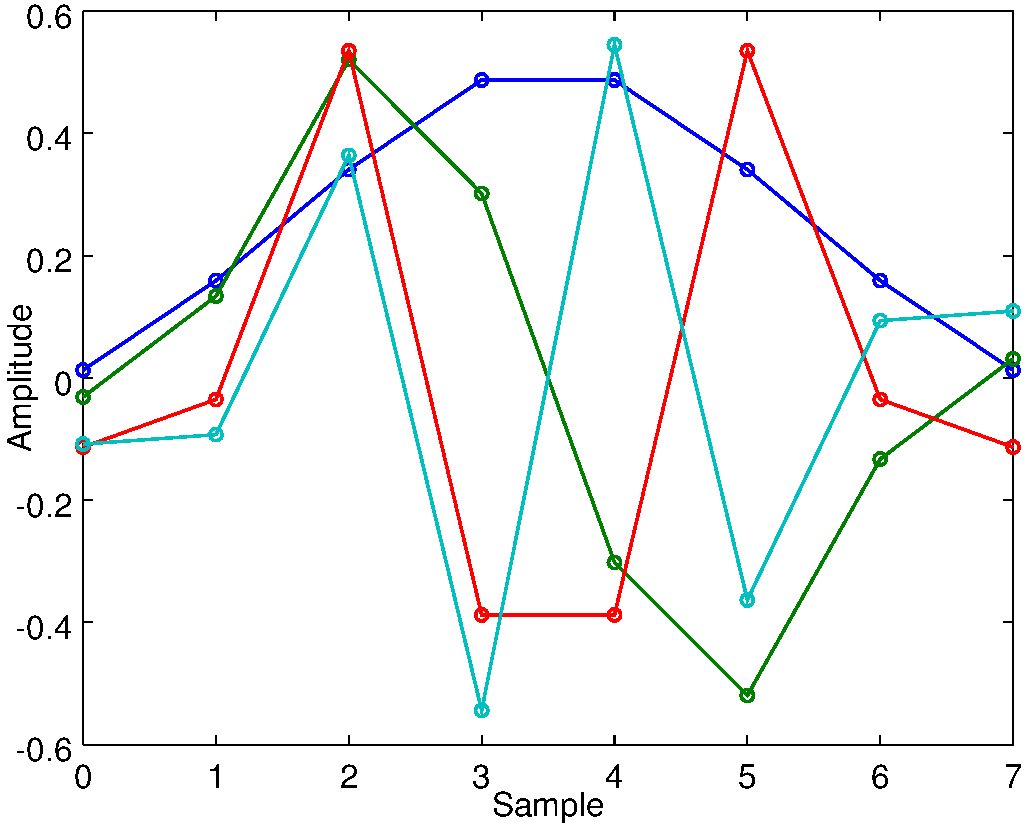
\includegraphics[width=0.8\columnwidth]{basis4}
\caption{1D synthesis basis functions for the lapped $4 \times 4$ DCT.\label{fig:basis4}}
\end{figure}

\subsection{Haar DC}
\label{sec:HaarDC}

Instead of using intra prediction for DC coefficients, the DC coefficients
within a superblock are further transformed with a 2D Haar wavelet.
Since Daala transform blocks are always split as quad-trees, the transform is
applied bottom-up, recursively, up to the level of the corresponding superblock,
as shown in \cref{fig:haardc}.
At each level, four DCs are combined into four Haar coefficients: one horizontal,
one vertical, one diagonal, and one new DC corresponding to a larger block size.

The highest level ($64\times 64$) DC is predicted as a linear combination of the
neighboring superblock DC coefficients: left, top-left, top, and top-right.
The prediction coefficients are trained on an image database and constrained to
sum to unity. The
(non-DC) horizontal and vertical Haar coefficients are predicted from
co-located horizontal and vertical coefficients at a larger scale. This slightly
reduces bitrate in smooth areas.

\begin{figure}
\centering
\begin{subfigure}[t]{0.49\columnwidth}
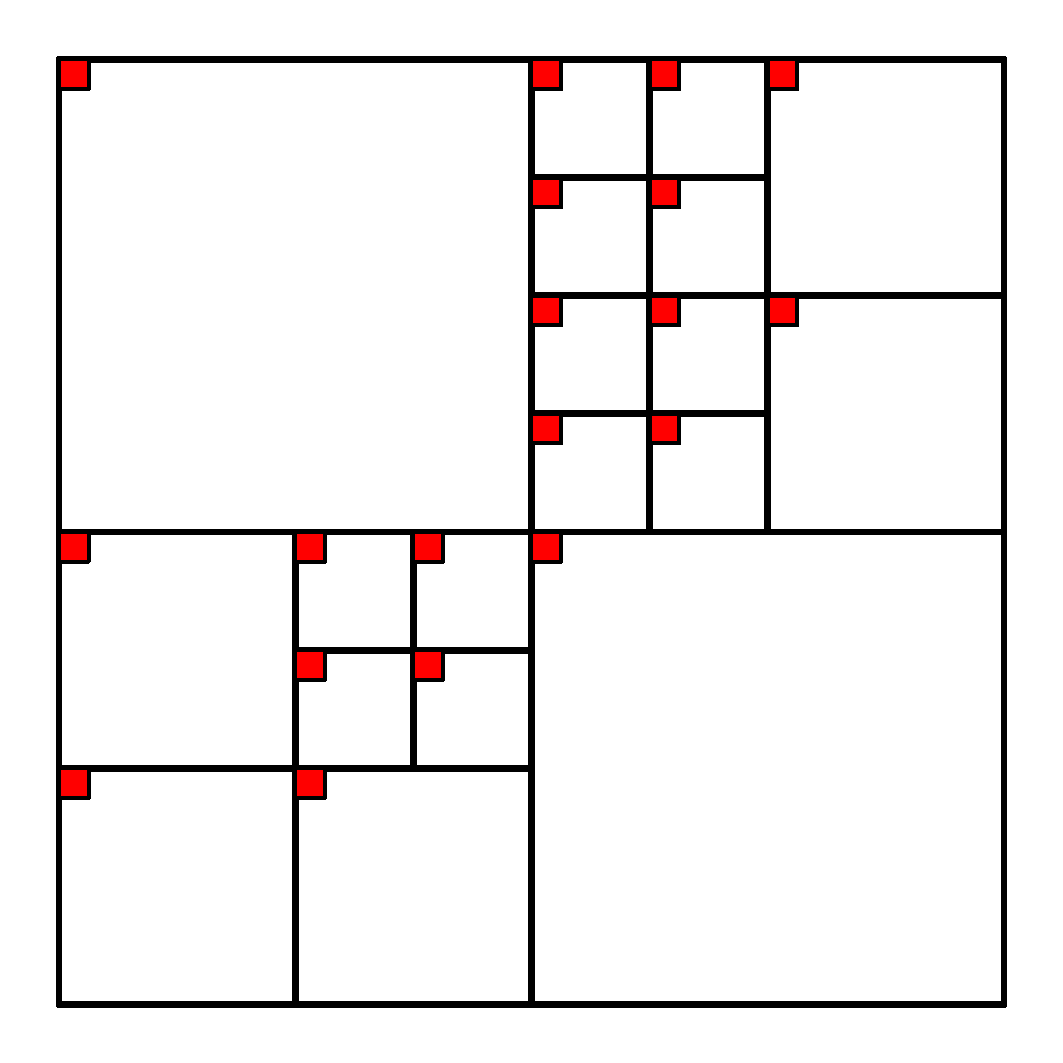
\includegraphics[width=\columnwidth]{block32_L0}
\caption{Original DC coefficients before Haar DC}
\end{subfigure}
\begin{subfigure}[t]{0.49\columnwidth}
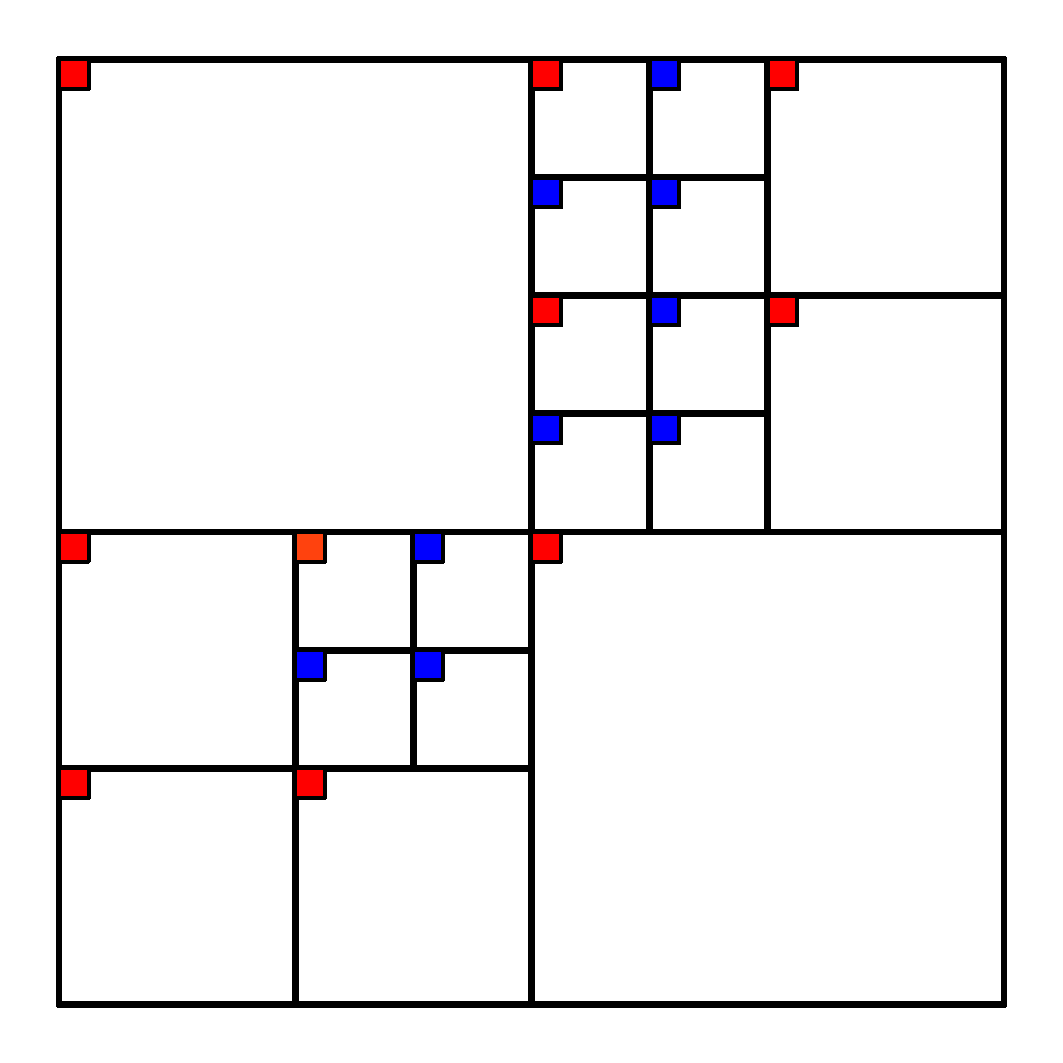
\includegraphics[width=\columnwidth]{block32_L1}
\caption{DC coefficients from $8\times 8$ blocks are combined}
\end{subfigure}
\begin{subfigure}[t]{0.49\columnwidth}
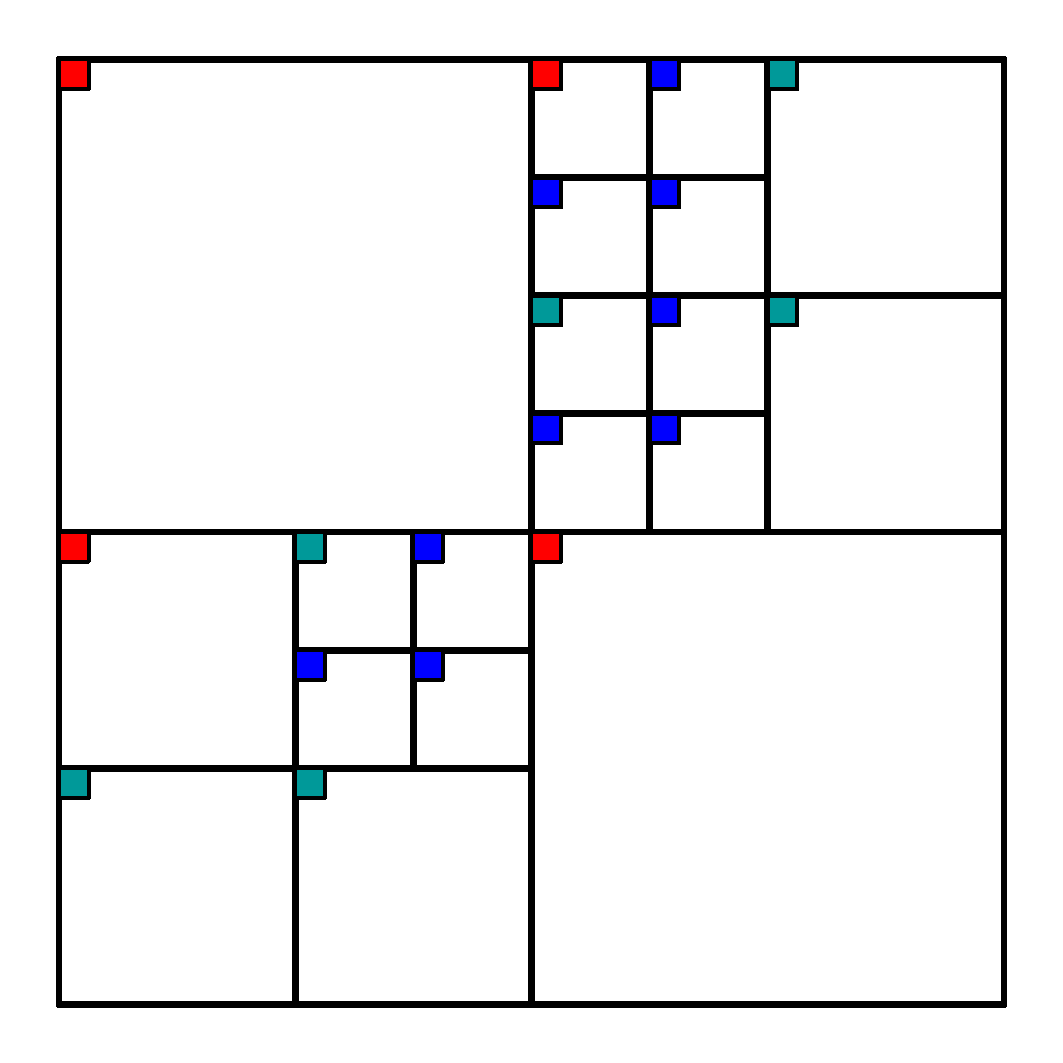
\includegraphics[width=\columnwidth]{block32_L2}
\caption{DC coefficients from $16\times 16$ sub-blocks are combined}
\end{subfigure}
\begin{subfigure}[t]{0.49\columnwidth}
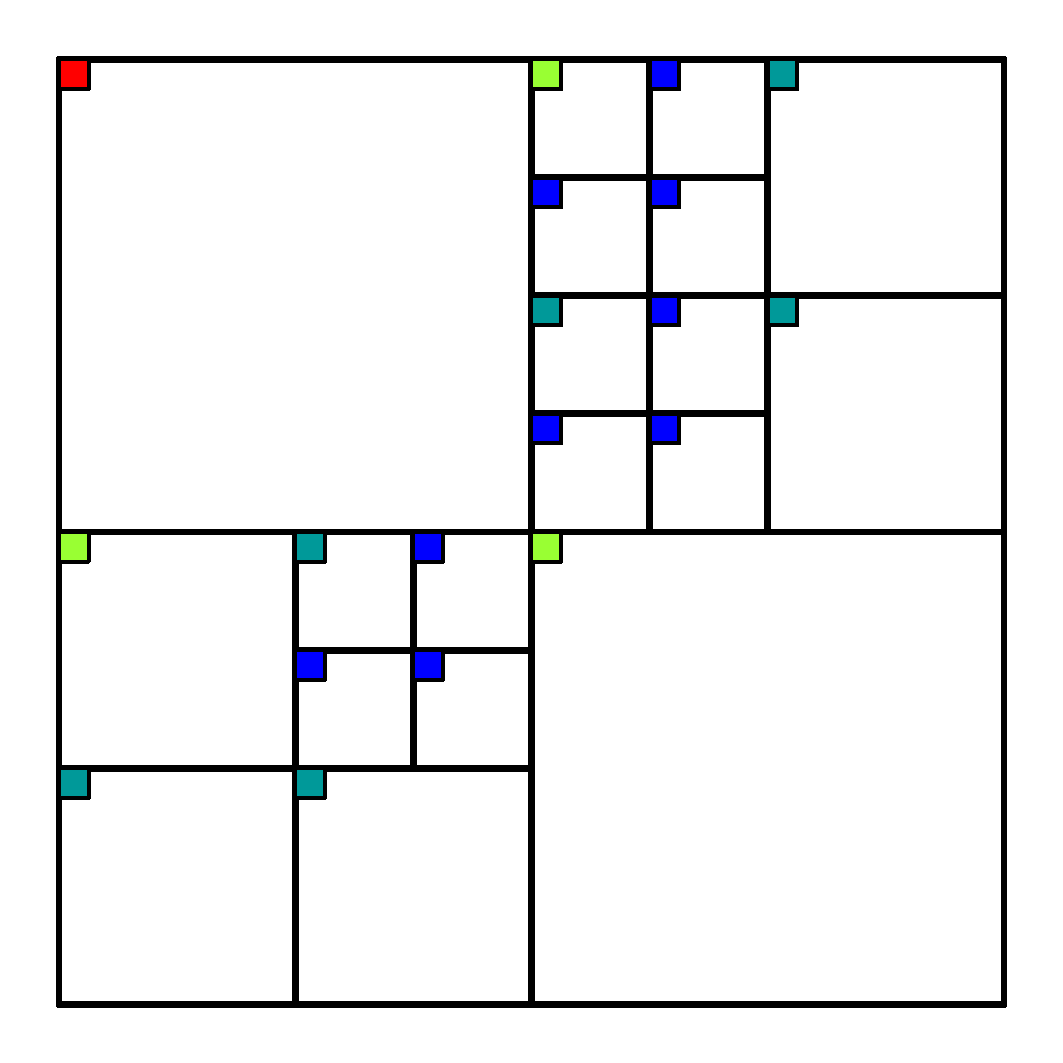
\includegraphics[width=\columnwidth]{block32_L3}
\caption{DC coefficients from $32\times 32$ sub-blocks are combined}
\end{subfigure}
\caption{Example of applying Haar DC over three levels on a $64\times 64$
superblock, subdivided into transform blocks of $8 \times 8$, $16 \times 16$,
and $32 \times 32$. At each step (a) to (d), the remaining DC coefficients
are shown in red\label{fig:haardc}}

\end{figure}

\subsection{Multi-Symbol Entropy Coder}
\label{sec:EntropyCoder}

Most recent video codecs encode information using binary arithmetic
coding, meaning that each symbol can only take two values. The Daala
range coder supports up to 16 values per symbol, making it possible
to encode fewer symbols~\cite{derfTools}. This is equivalent to
coding up to four binary values in parallel and reduces serial dependencies,
allowing hardware implementations to use lower clock rates, and thus less
power.

The range coder itself is based on a multiply-free approximation presented
in~\cite{stuiver1998piecewise}. The original approximation overestimates
probabilities for symbols at the end of the alphabet, and underestimates
probabilities at the beginning of the alphabet. In Daala, this is done the
other way around, since $0$ is frequently the most probable symbol.
Overestimating its probability leads to lower approximation overhead than
underestimating it.

The approximation replaces the multiplication and division of a traditional
arithmetic coder with a subtraction, a minimum operation, and an addition. This
allows it to work with any input probability distribution, without requiring
that its total be normalized to a power of two. That lets Daala use traditional
frequency counts to model probabilities, instead of having to extend the
table-based schemes usually used by binary coders to larger alphabet sizes.
Probabilities can typically be updated with just one or two SIMD instructions
in software, and are similarly cheap to update in parallel in hardware. The
overall cost of the approximation is a bitrate of around $1\%$ in practice,
which is comparable to CABAC\@.

We are currently exploring approaches for reducing this overhead without
sacrificing throughput or modeling efficiency with hardware implementers in the
AOM\@.

\subsection{Overlapped Block Motion Compensation}
\label{sec:OBMC}

Because hard block edges are expensive to code with lapped transforms, we
want to avoid creating blocking artifacts in the motion-compensated
prediction. For this we use overlapped block motion compensation
(OBMC)~\cite{OBMC}. This is done on an adaptive grid of Motion Compensation
(MC) blocks ranging from $8\times 8$ up to $64\times 64$, in order to scale to
high-resolution content. This grid is completely independent of the transform
blocks, and neither imposes any constraints on the sizes of the other. We also
experimented with $4\times 4$ blocks, but they were rarely used in practice,
and actually caused a small quality regression at equal bitrate with the
encoder used at the time.

The use of variable-sized MC blocks requires a blending scheme that maintains
continuity between neighboring regions of different sizes. One approach, used
by codecs like Dirac~\cite{Dirac}, is to fix the overlap size at the largest
overlap allowed by the smallest motion compensated block (8~pixels, in this
case). This makes a large
block equivalent to a group of smaller blocks with the same motion vector.
However, this can create low-passing artifacts in a predictable grid pattern.
These can be visually annoying, and require many bits to correct because of
their locality. Zhang \textit{et al.} showed that splitting large blocks,
but only as far as necessary to prevent their blending windows from
overlapping more than one neighboring block, improved quality~\cite{ZAS98}.
However, they implemented this as a post-process to a non-overlapped
block-based motion search, and did not incorporate RDO\@.

Instead, Daala structures its grid as a 4-8 mesh~\cite{DWSMAM97} to ensure the
sizes of neighboring MC blocks differ by no more than a factor of two. This
makes it easy to design OBMC blending windows that both span an entire block
and ensure continuity across block size changes. Although R-D optimal block
size decisions with this data structure are still NP-hard, there is a fast
dynamic programming approximation that achieves good results in
practice~\cite{Bal01}. The details of the 4-8 grid structure, the blending
windows, and the dynamic programming algorithm are outlined in~\cite{OBMC}.

\subsection{Perceptual Vector Quantization}
\label{sec:PVQ}

In the majority of video codecs, a motion-compensated reference frame
is subtracted from the input frame to compute a residual, which is
then transformed, and coded using scalar quantization. Daala differs
significantly from that description. Not only does it use vector quantization
rather than scalar quantization, but --- most importantly --- the motion-compensated
reference is never subtracted from the input frame. Instead,
the motion-compensated reference is used to build a transformation
that makes the input easier to code. This technique is called perceptual
vector quantization (PVQ)~\cite{valin2015spie}.

Perceptual vector quantization originates in the pyramid vector quantizer
previously used for music in the Opus audio codec~\cite{ValinAES}. In Opus,
the pyramid vector quantizer is used as a gain-shape quantizer in a way that
ensures that the signal energy is always conserved. Using a gain-shape
quantizer in a video codec is more complicated, since we need to also take
into account a prediction. While it would be possible to quantize the
scalar difference
between the prediction and the input, conserving the energy of that
difference would be perceptually meaningless.

Rather than attempting to encode the difference, the prediction produces
a Householder reflection that makes the input easier to encode. Let
$\mathbf{x}$ be the input and $\mathbf{r}$ be the prediction, we construct
 a Householder reflection plane
\begin{equation}
\mathbf{v} = \frac{\mathbf{r}}{\|\mathbf{r}\|} + s\mathbf{e}_m\ ,
\end{equation}
where $\mathbf{e}_m$ is a unit vector along dimension $m$ and $s = \pm1$.
The values of $m$ and $s$ can be chosen arbitrarily, but to maximize
numerical stability, we typically choose $m$ to be the position of the
largest absolute value in $\mathbf{r}$ and $s$ to be the sign of that value.

Once the reflection plane is computed, it is applied to the input vector
$\mathbf{x}$ to produce the reflected vector $\mathbf{z}$:
\begin{equation}
\mathbf{z} = \mathbf{x} - 2\frac{\mathbf{x}^T\mathbf{v}}
{\mathbf{v}^T\mathbf{v}}\mathbf{v}\ .
\end{equation}
When the input is similar to the prediction itself, the direction of the
reflected vector $\mathbf{z}$ is close $-\mathbf{e}_m$. To take advantage of
that fact, we express it as
\begin{equation}
\mathbf{z} = g\left(-s\cos\theta + \mathbf{u}\sin\theta\right)\ ,
\end{equation}
where $g$ is the magnitude of $\mathbf{z}$ (and thus also the magnitude of
$\mathbf{x}$), $\mathbf{u}$ is a unit vector with no component along the
$\mathbf{e}_m$ direction, and $\theta$ is the angle between $\mathbf{r}$ and
$\mathbf{x}$ (a meaningful parameter that represents the similarity between
the prediction and the input). Since the Householder reflection is orthonormal,
it follows that
\begin{equation}
\theta = \arccos\frac{\mathbf{x}^T\mathbf{r}}
                   {\left\|\mathbf{x}\right\|\left\|\mathbf{r}\right\|}\ .
\end{equation}

The unit vector $\mathbf{u}$ can be coded using a spherical quantizer derived
from the pyramid vector quantizer~\cite{Fischer1986}:
\begin{equation}
\mathbf{u}=\frac{\mathbf{y}}{\left\|\mathbf{y}\right\|}\ ,
\end{equation}
with
\begin{equation}
\mathbf{y} \in \mathbb{Z}^N : \left\|\mathbf{y}\right\|_{L1} = K \land y_m=0\ ,
\end{equation}
where the number of \textit{pulses} $K$ controls the size of the codebook.

The encoder quantizes $g$ and $\theta$ and encodes them in the bitstream along
with the integer vector $\mathbf{y}$ (except for $y_m=0$). The codebook
size $K$ is determined only from $g$ and $\theta$ and does not need to be
transmitted. Since the decoder has access to the prediction vector $\mathbf{r}$,
it can compute the reflection vector $\mathbf{v}$ without the need to transmit
$m$ and $s$. In total, there are $N-2$ degrees of freedom to code in
$\mathbf{y}$, with two more for $g$ and $\theta$, so the total is still
$N$ degrees of freedom. The main difference however is that two of the
coded values have a perceptual meaning: $g$ is the amount of contrast and
$\theta$ is the amount of change compared to the prediction. By coding $g$
as a parameter, it is easier to preserve the amount of contrast than by
coding only DCT coefficients.

In practice, the vectors $\mathbf{x}$ and $\mathbf{r}$ are transform
coefficients rather than pixel values. This requires an extra forward DCT
in both the encoder and the decoder since the input and the prediction need
to be transformed separately. Only the AC coefficients are coded using PVQ
and for transform blocks larger than $4\times 4$, the AC coefficients are divided into multiple
\textit{bands} where each band is coded separately. This makes it possible
to control the contrast separately, based on octave and direction.

PVQ makes it possible to take into account masking effects with no
extra signaling. Since the gain is explicitly signaled, it is easy to make
the quantization resolution dependent on the gain. This dependency can be
expressed as
\begin{equation}
E\left\lbrace \left\| \mathbf{x} - \hat{\mathbf{x}} \right\|^2 \right\rbrace
\propto g^{2\alpha}\ , 0 \leq \alpha \leq 1\ ,
\end{equation}
where $\alpha=0$ behaves like a standard linear scalar quantizer and
$\alpha=1$ produces a constant relative error like in the Opus audio codec.
Daala uses $\alpha = \nicefrac{1}{3}$. To achieve this, we quantize the
companded gain
\begin{equation}
\gamma = g^{1-\alpha}\ ,
\end{equation}
giving finer resolution to smaller gains and coarser resolution to larger
gains.

The decoder always decodes the quantized companded gain $\hat{\gamma}$
first. From there it can compute the quantization step size for $\theta$ as
\begin{equation}
Q_\theta = \frac{\beta}{\hat{\gamma}}\ ,
\end{equation}
where $\beta = \frac{1}{1-\alpha}$.

The size of the codebook $K$ was determined through curve
fitting~\cite{valin2015spie} to be
\begin{equation}
K = \frac{\hat{\gamma}\sin\hat{\theta}}{\beta}\sqrt{\frac{N+2}{2}}\ .
\label{eq:K_nonrobust}
\end{equation}
The formulation in~\cref{eq:K_nonrobust} is not robust to packet loss when
the gain is predicted (leading the decoder to obtain the wrong $K$ and decode
the wrong number of symbols). Fortunately, by making the $\sin{\hat{\theta}}
\simeq \hat{\theta}$ approximation and substituting $\hat{\theta} =
Q_\theta\hat{\tau}$, where $\hat{\tau}$ is the angle quantization index, we obtain
\begin{equation}
K = \hat{\tau} \sqrt{\frac{N+2}{2}}\ .
\end{equation}


\subsection{Chroma from Luma (CfL) Prediction}
\label{sec:CFL}
Although the use of $\mathrm{Y'C_BC_R}$ reduces the correlation across planes
compared to RGB, there still exists a correlation between the chroma planes
$\mathrm{C_B}$ and $\mathrm{C_R}$ and the luma plane $\mathrm{Y'}$. Edges in
chroma tend to
align very well with edges in luma with only the amount of contrast (gain) differing.
Because of that property, PVQ makes it especially easy to predict
chroma planes from the luma plane. Daala's chroma from luma (CfL)~\cite{egge2015spie}
prediction directly uses the luma transform coefficients as the prediction vector
$\mathbf{r}$ for coding the chroma coefficients with PVQ\@. The main difference compared
to the normal way of using PVQ is that a sign needs to be coded for the prediction
(since the luma plane and chroma plane coefficients may be negatively correlated) and
that the gain of the chroma cannot be predicted from the gain of the luma.


\subsection{Directional Deringing Filter}
\label{sec:deringing}

Like other transform codecs, Daala can cause ringing artifacts around edges.
The directional deringing filter attempts to eliminate the ringing without
blurring the image. Unlike the HEVC Sample-Adaptive Offset (SAO)~\cite{HEVC-SAO},
the Daala deringing filter is not based on classifying pixels and applying per-class
offsets. Instead, it is a directional outlier-robust filter that smooths the
neighborhood of pixels while preserving edges.

Let $x\left(n\right)$ denote a 1-dimensional signal and $w_{k}$
denote filter tap weights. A linear finite impulse response (FIR)
filter with unit DC response is defined as
\begin{equation}
y\left(n\right)=\frac{1}{\sum_{k}w_{k}}\sum_{k}w_{k}x\left(n+k\right)\ ,\label{eq:FIR1}
\end{equation}
which can alternatively be written as
\begin{equation}
y\left(n\right)=x\left(n\right)+\frac{1}{\sum_{k}w_{k}}\sum_{k,k\neq0}w_{k}\left[x\left(n+k\right)-x\left(n\right)\right]\ .\label{eq:FIR2}
\end{equation}
The main advantage of expressing a filter in the form of~\cref{eq:FIR2}
is that the normalization term $\frac{1}{\sum_{k}w_{k}}$ can be approximated
relatively coarsely without affecting the unit gain for DC\@. This makes
it easy to use small integers for the weights $w_{k}$.

The disadvantage of linear filters for removing ringing artifacts
is that they tend to also cause blurring. To reduce the amount of
blurring, the conditional replacement filter used in Daala excludes
the signal taps $x\left(n+k\right)$ that would cause blurring and
replaces them with $x\left(n\right)$ instead. This is determined
by whether $x\left(n+k\right)$ differs from $x\left(n\right)$ by
more than a threshold $T$. The FIR filter in~\cref{eq:FIR2}
then becomes a conditional replacement filter expressed as
\begin{equation}
y\left(n\right)=x\left(n\right)+\frac{1}{\sum_{k}w_{k}}\sum_{k,k\neq0}w_{k}R\left(x\left(n+k\right)-x\left(n\right),T\right)\ ,\label{eq:CRF}
\end{equation}
where
\begin{equation}
R\left(x,T\right)=\left\{ \begin{array}{ll}
x & ,\ \left|x\right|<T\\
0 & ,\ \mathrm{otherwise}
\end{array}\right.\ .
\end{equation}

To further reduce the risk of blurring the decoded image, the conditional
replacement filter is applied along the main direction of the edges
in each $8\times 8$ transform block. The direction is determined based on the decoded image
(no side information transmitted) by analyzing each $8\times 8$ block as described
in~\cite{ValinDeringing}. For each $8\times 8$ block, the decoder determines which
of eight different directions best represents the content of the block.
The search can be efficiently implemented in SIMD\@. To filter a pixel, a 7-tap
conditional replacement filter is applied along the detected direction.
The process is repeated for each pixel in each block being filtered.

To further reduce ringing in very smooth regions of the image, the filter
is applied a second time to combine multiple output values of the
first filter. The second filter is applied either vertically or horizontally
-- in the direction most orthogonal to the one used in the first filter.
For example, for a 45-degree direction, the second filter would be
applied horizontally. The combined effect of the two filters is a separable
deringing filter that covers a total of 35~pixel taps.

The deringing filter only requires a minimal amount of signaling. A global threshold
is set for the entire a frame, and one of six adjustment factors (including an
\textit{off} setting) is signaled for each superblock. With entropy coding, the
cost of the signaling generally averages 2~bits per superblock, or 128~bytes for
a 1080p keyframe. For predicted frames, the deringing filter is not applied to
$8\times 8$ blocks where no coefficients are coded, and no adjustment factor
is coded for superblocks where no $8\times 8$ block is filtered, further
reducing the amount of signaling. The
effect of the deringing filter at low bitrate is shown in \cref{fig:deringing}.

\begin{figure}
\centering
\begin{subfigure}[t]{0.5\columnwidth}
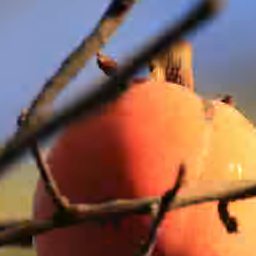
\includegraphics[width=\columnwidth]{fruits_nodering_crop}
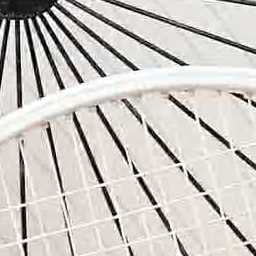
\includegraphics[width=\columnwidth]{bike_nodering_crop}
\caption{Without deringing filter}
\end{subfigure}\begin{subfigure}[t]{0.5\columnwidth}
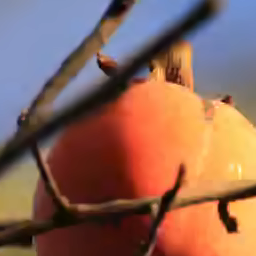
\includegraphics[width=\columnwidth]{fruits_dering_crop}
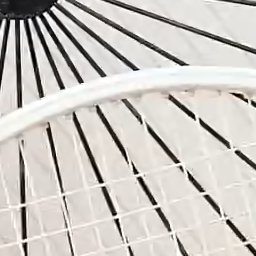
\includegraphics[width=\columnwidth]{bike_dering_crop}
\caption{With deringing filter}
\end{subfigure}
\caption{Effect of the deringing filter on two images with sharp edges.\label{fig:deringing}}
\end{figure}

\section{Alliance for Open Media AV1 codec}
\label{sec:AOM}

The recently-formed Alliance for Open Media (AOM) is currently specifying
AV1, a royalty-free video codec. The initial development is based on
technology from three existing codecs: Google's VP9~\cite{VP9Spec} codec,
Cisco's Thor~\cite{ThorDraft} codec, and the Daala codec presented
here. For this reason, some of the techniques used in Daala are currently
being considered for inclusion in AV1.

The deringing filter described in \cref{sec:deringing} is already
fully integrated in AV1 and has been shown to reduce bitrate by around 2\%
at equal quality. AV1 also includes Thor's constrained lowpass
filter~(CLPF)~\cite{CLPFDraft} that attenuates ringing, but with a more
limited effect and a lower complexity than the Daala deringing filter.

The multi-symbol entropy coder (\cref{sec:EntropyCoder}) is also being
evaluated. Using the piecewise
integer mapping exactly as described in~\cite{stuiver1998piecewise} results
in a bitrate overhead of around 1\%. However, we have experimented with
better approximations that do not have such cost and assume that
the denominator of the probabilities is a power of two.

PVQ (\cref{sec:PVQ}) is early stages of experiments in AV1 and is by far
the most invasive
of the Daala techniques under consideration in AV1, as it requires many changes
in the signaling, as well as the addition of a forward transform on the
prediction itself. No results are available yet, but should PVQ be
included in AV1, it would make it possible to also experiment with CfL
(\cref{sec:CFL}).

Lapped transforms (\cref{sec:lapping}) and OBMC (\cref{sec:OBMC}) are 
\textit{not} being considered for inclusion
in AV1. Both these techniques have far-reaching interactions with the
other coding techniques and would essentially require a complete re-design
of the codec. Considering that Haar~DC (\cref{sec:HaarDC}) is mostly
needed to compensate for the
lack of pixel-domain prediction, it also not currently being considered for AV1.

\section{Results and Discussion}
\label{sec:Results}

\begin{figure*}
\centering
\begin{subfigure}[t]{0.5\textwidth}
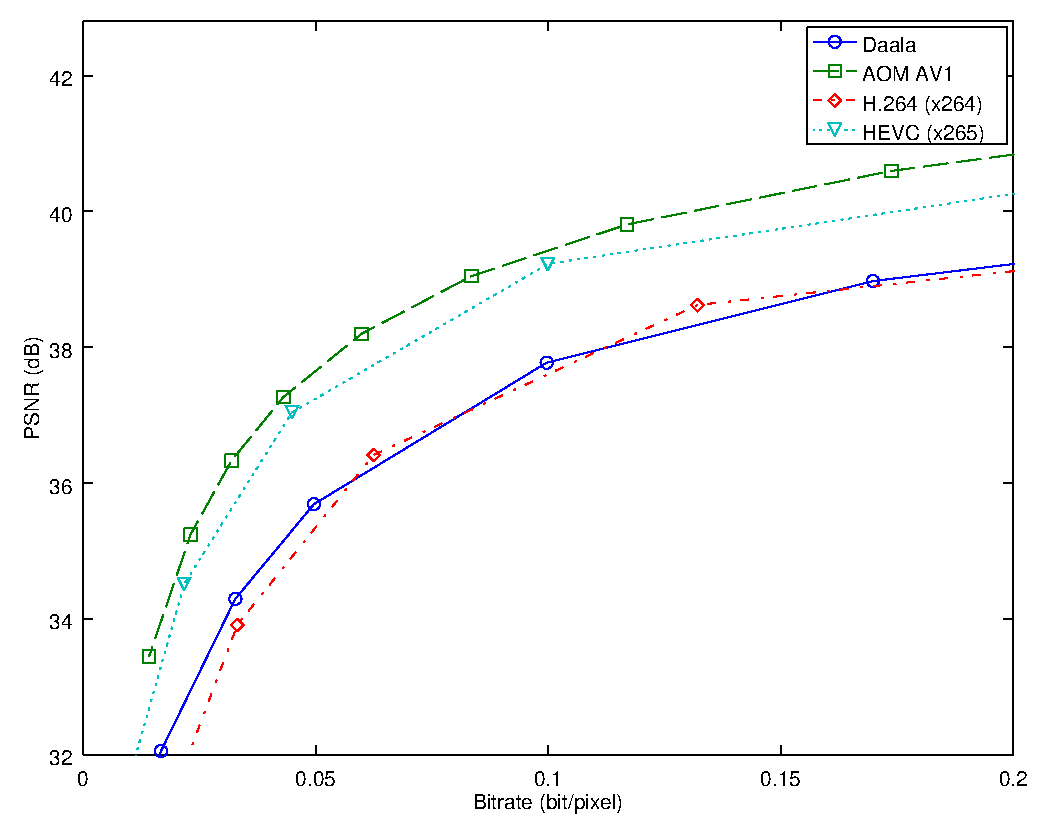
\includegraphics[width=\columnwidth]{psnr.eps}
\caption{PSNR}
\end{subfigure}\begin{subfigure}[t]{0.5\textwidth}
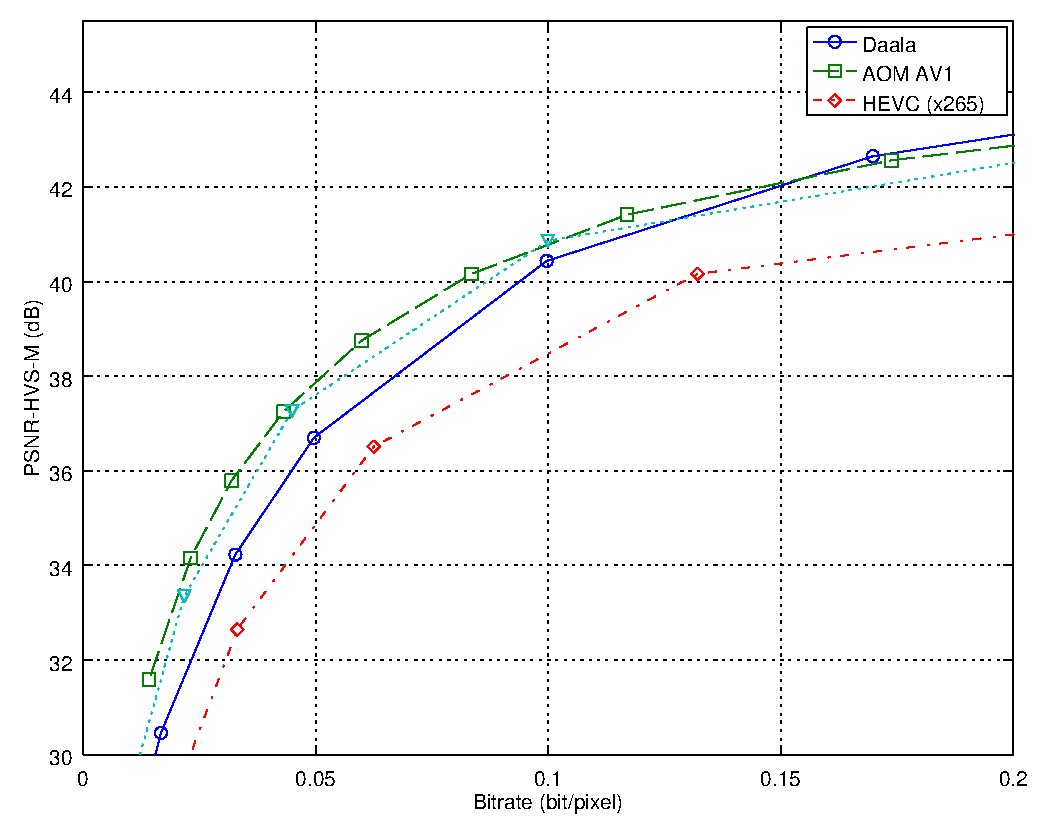
\includegraphics[width=\columnwidth]{psnrhvsm.eps}
\caption{PSNR-HVS-M}\label{fig:psnrhvsm}
\end{subfigure}
\begin{subfigure}[t]{0.5\textwidth}
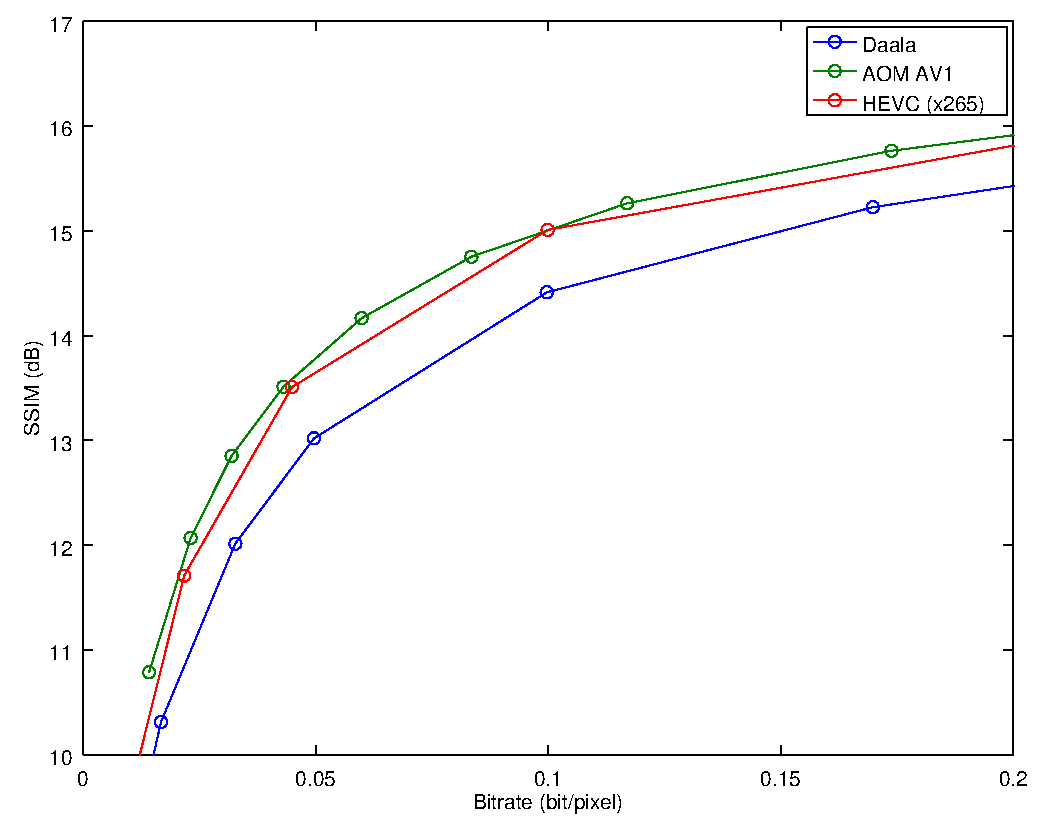
\includegraphics[width=\columnwidth]{ssim.eps}
\caption{SSIM}
\end{subfigure}\begin{subfigure}[t]{0.5\textwidth}
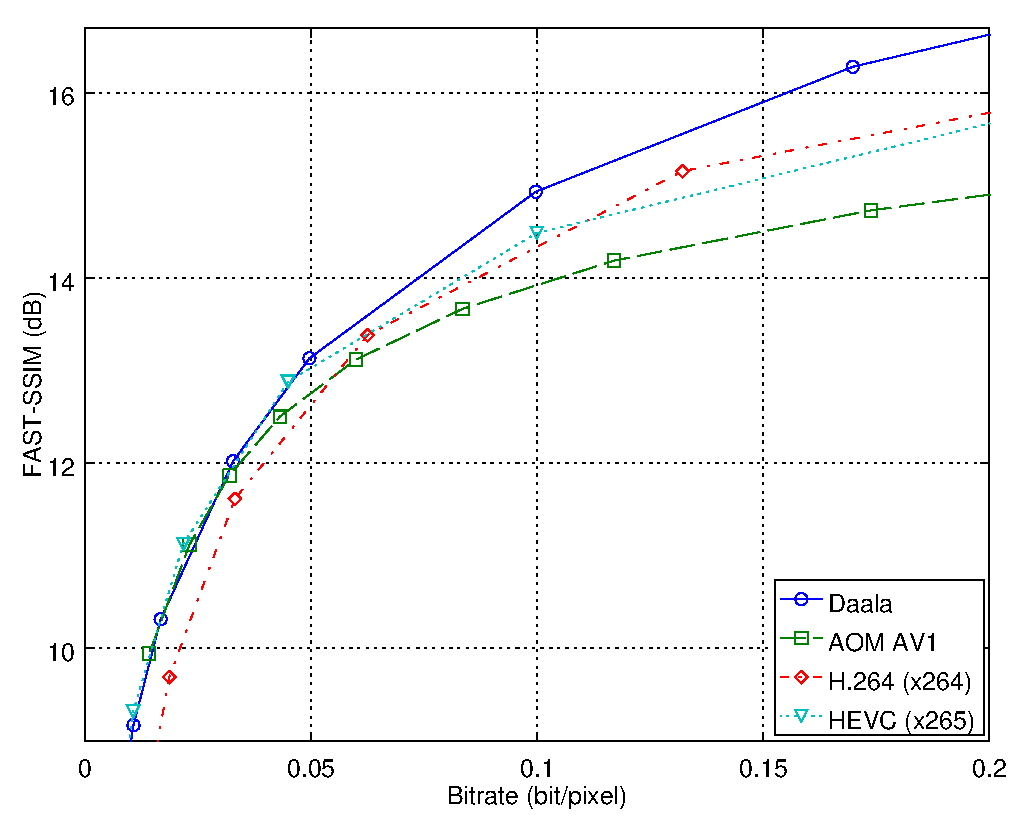
\includegraphics[width=\columnwidth]{fastssim.eps}
\caption{FAST-SSIM}
\end{subfigure}
\caption{Comparison between Daala, HEVC and AV1 based on objective metrics.}\label{fig:metrics}
\end{figure*}

Testing of Daala is performed on the Are We Compressed 
Yet?\footnote{\url{https://arewecompressedyet.com/}} testing infrastructure
on the \texttt{ntt-short-1} test set.
Four different objective metrics are used for the comparison: PSNR,
PSHR-HVS-M~\cite{PSHRHVSM}, SSIM, and Fast-SSIM~\cite{FastSSIM}. We compare
Daala\footnote{Git version d55fff01 from April 25th, 2016 with command-line options: -k 1000 -v}
to the AV1 encoder\footnote{Git version 337b23a5 from April 7th, 2016 with deringing enabled and command-line options: --ivf --frame-parallel=0 --tile-columns=0 --auto-alt-ref=2 --cpu-used=0 --passes=2 --threads=1 --kf-min-dist=1000 --kf-max-dist=1000 --lag-in-frames=25 --end-usage=q --cq-level=}, to the x264 H.264
encoder\footnote{Command-line options: --preset placebo --min-keyint 1000 --keyint 1000 --no-scenecut --crf=},
and to the x265 HEVC encoder\footnote{Version 1.6 with command-line options: --preset slow --frame-threads 1 --min-keyint 1000 --keyint 1000 --no-scenecut --crf=}.

The results in \cref{fig:metrics} show that Daala is generally better than
H.264, but worse than HEVC and AV1. From the developers' informal
evaluation, the subjective performance of Daala is close to what the PSNR\-HVS\-M
results show in \cref{fig:psnrhvsm}. Qualitatively, the Daala artifacts tend to differ
greatly from most other video codecs. Daala tends to perform more poorly on sharp
details and edges, while retaining more of the smooth texture. This is in part due
to the PVQ activity masking, but the behavior is present even when activity masking
is not used.

Considering that most of the technology used in Daala is either new or unproven
in the context where it is being used, we consider these results to be
encouraging. Some of the techniques presented in this paper should make their
way into the AV1 codec, with others will require more time to mature before
being used in a video coding standard.

\bibliographystyle{IEEEtran}
\bibliography{daala}

\end{document}
